\documentclass[11pt,a4paper]{article}

\usepackage{titling}
\usepackage[hidelinks]{hyperref}
\usepackage{graphicx}
\usepackage{grffile}
\usepackage{float}
\usepackage{geometry}
\usepackage{listings}

\newcommand{\subtitle}[1]{
  \posttitle{
    \par\end{center}
    \begin{center}\large#1\end{center}
    \vskip0.5em}
}

\begin{document}


\title{Hyper Perform\\ Testing Document}
\subtitle{ Organisation: \url{https://github.com/Hyperperform}}
\begin{figure}
			\centering
			
\includegraphics[height=200px]{../Images/CodusMaximus_logo.jpg}
\end{figure}

	
\author{
	\textbf{Developers:} \\
	Claudio Da Silva	\emph{14205892}	\\
	Rohan Chhipa		\emph{14188377}	\\
	Avinash Singh		\emph{14043778}	\\
	Jason Gordon		\emph{14405025}	\\\\
}

\date{\textbf{Updated \today}}

\maketitle
\thispagestyle{empty}
\pagebreak

\tableofcontents
\pagebreak

\section{Introduction}

This document explains implementation of unit tests which were used to test each component in an isolated environment. It also includes an overview of the technologies used as well as instructions on how to execute these tests. \\ 

\section{Purpose}
The HyperPerform system was made to be able to track employee performance. One of the main goals of the system is to be able to use the system in any industrial or academic field. To ensure this each component of the system is decoupled from every other. All aspects of the system are implemented such that they conform to the given contracts. Unit testing is essential to ensure that these contracts are not violated in anyway and to ensure that the components that expose the services (REST wrapping) are all working properly before the system is deployed.

\section{Technologies}

Since the system was primarily coded with Java we used JUnit to carry out the unit tests for each of the components. We also used Spring to allow us to use dependency injection within each test, this allows us to easily inject mocks and test components in an isolated environment. \\\\
Another technology which proved useful was a Mock Dispatcher framework which ships with RESTEasy. The mock dispatcher allows one to easily and efficiently test REST API's without having to deploy the component to an application server.

\section{Testing environment}
\begin{itemize}
	\item \textbf{Programming Languages:} Java with JavaEE for the back-end server, front-end relies on AngularJS with Bootstrap.
	\item \textbf{Testing frameworks: } Unit testing is done using JUnit.
	\item \textbf{Operating System: } The system is designed for any operating system provided the correct software is correctly setup. This system was developed in Linux OS. The system will also have Docker for easy of usage.
	\item \textbf{Internet Browsers: } The front-end system supports the latest versions of 
	$Google Chrome$ and $Firefox$. There is limited support for other browsers.
\end{itemize}

\section{Execution of unit tests}	
The project was developed using Maven as a build tool. Unit tests Thus each unit test can be easily found within the $src/test$ directory of the project. To run the unit tests simply run the following command on terminal: \\

$mvn\ clean\ test$ \\\\
All the necessary dependencies for the project will be automatically downloaded. \textbf{Note:} This process of downloading all the project dependencies might consume large amounts of data and time.

\section{Test items}
At this point in the project the following features have been tested:
\begin{itemize}
	\item GitListener which receives events from GitHub.
	\item GitPushEvent which is a POJO that contains information regarding a GitHub event.
	\item CalendarListener which receives events from Google Calendar service.
	\item CalendarMeeting which is a POJO that contains information of Meetings from Google Calendar.
	\item CalendarProject which is a POJO that contains information of Projects from Google Calendar. 
	\item TravisListener which receives events from Travis CI.
	\item TravisEvent which is a POJO that contains information regarding a build triggered by a push event from GitHub
	\item AccessEvent which is a POJO that contains information of access in/out of a building containing a card reader.
	\item The error codes and exceptions raised when accessing an invalid REST URL.
	 
\end{itemize}

Mock JSON data has been passed to the GitListener and CalendarListener classes (into the listen functions). \\\\
Each of these components have dependencies on features such as the messaging queue. All of these features are mocked out to ensure each component is tested in isolation. These features were mocked through dependency injection which was provided by Spring. \\

\section{Features that will not be tested}

Features that have been provided by frameworks will not be tested. Operations such as adding an object to a messaging queue will not be tested. Mapping of JSON data to request objects as this is also done by frameworks.

\section{Components to be mocked}
\begin{itemize}
	\item The JPA entity manager was the first component that was mocked. When testing the possibility for persistence of the POJO's it would be best if the transactions do not affect the database. Thus every transaction that occurs with the mocked entity manager will leave the database system intact and unaffected. An alternate approach could have been to use an in-memory database - such as the one provided by H2 - however this was not deemed necessary. \\
	
	\item The second component to be mocked was the messaging queue provided by ActiveMQ. Once again we do not wish to have unnecessary objects in our queue that might affect actual program execution thus the default queue is replaced with a queue that does not retain objects. \\
	
	\item When testing the event listeners we can't wait for the event emitting systems to send out an event. So we send mock events to the listeners while testing, these mock events are structured in the same manner as there real-world counterparts.
\end{itemize}

\section{Sample tests}
The following figure is the GitListener dependency injected queue which allows multiple events to come through and not be lost and the creation of the entity manager.
\begin{figure}[H]
	\begin{center}
		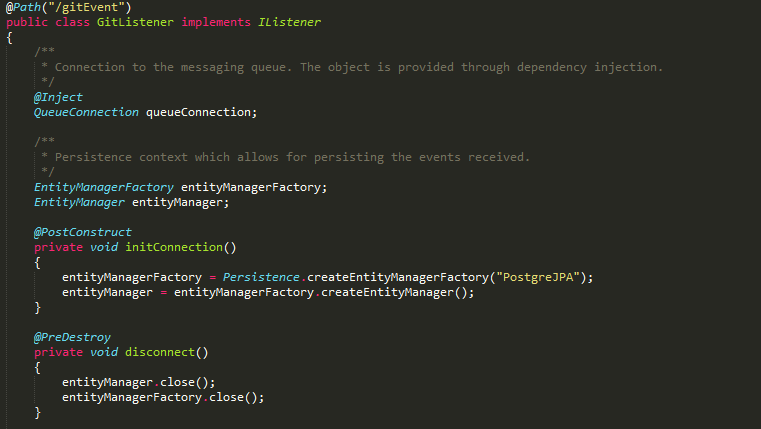
\includegraphics[scale=0.7]{../Images/sample3.PNG}
		\caption{GitListener Dependency injection}
	\end{center}
\end{figure}


The following figure is one of the GitListener Event tests.

\begin{figure}[H]
	\begin{center}
		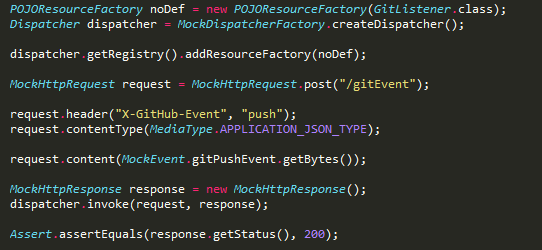
\includegraphics[scale=1.0]{../Images/sample1.PNG}
		\caption{GitListener Push event test}
	\end{center}
\end{figure}
\noindent
In the above figure the $POJOResourceFactory$ and $Dispatcher$ are used to start up an embedded server which will allow for calls to be made to a particular URL, in this case $\backslash$ gitEvent. \\
\\
A post request is created and has the mock event as its content. This post request mirrors the post requests made by GitHub when sending events. Once the mock event data is loaded into the request, the request is sent. At the end, the response objects' HTTP status code is checked. This is checked in an assert statement, the value of the response should be 200 to indicate a successful retrieval. \\

\begin{figure}[H]
	\begin{center}
		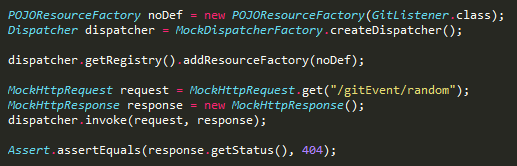
\includegraphics[scale=1.0]{../Images/sample2.PNG}
		\caption{Exception handler for invalid URLs}
	\end{center}
\end{figure}


\section{Unit Test Report}
\subsection{Overview}
All the test of the system has passed and the reason that a test may fail is if the database tables are not created properly as these tables are not created using JPA, since JPA destroys and creates the tables upon the command used for testing $mvn clean test$. We use Travis CI for our builds to ensure that all the build pass.

\subsection{Test Cases}

\subsubsection{Test Class 1}
	\url{https://github.com/HyperPerform/hyper-perform-server/blob/develop/src/test/java/me/hyperperform/event/CalendarPersistenceTest.java}\\\\
 \textbf{CalendarPersistenceTest}
 \begin{itemize}
 	\item $jpaTest$ - Test if the CalendarMeeting and CalendarProject POJOS persist.
	\item $QueryTest$ - Test to see if the persisted objects were actually persisted properly and check the data integrity.\\
\end{itemize}
Result: \textbf{All Passed}


\subsubsection{Test Class 2}
\url{https://github.com/HyperPerform/hyper-perform-server/blob/develop/src/test/java/me/hyperperform/event/DatabasePopulatorTest.java}\\\\
\textbf{DatabasePopulatorTest}
\begin{itemize}
	\item $databasePopTest$ - This test is to insert mock data for all the tables into the database so that relevant reports can be generated.\\
\end{itemize}
Result: \textbf{All Passed}


\subsubsection{Test Class 3}
\url{https://github.com/HyperPerform/hyper-perform-server/blob/develop/src/test/java/me/hyperperform/event/PersistenceTest.java}\\\\
\textbf{PersistenceTest}
\begin{itemize}
	\item $queryTest$ - This creates a GitPush POJO and persists it thereafter query the database and check data integrity.
	\item $gitIssuePojoTest$ - This creates a GitIssue POJO and persists it.
	\item $travisPojoTest$ - This creates a TravisEvent POJO and persists it.\\

\end{itemize}
 Result: \textbf{All Passed}


\subsubsection{Test Class 4}
\url{https://github.com/HyperPerform/hyper-perform-server/blob/develop/src/test/java/me/hyperperform/rest/RestTest.java}\\\\
\textbf{RestTest}
\begin{itemize}
	\item $gitIssueEventTest$ - Uses MockEvent.gitIssuesEvent JSON data for issues and tests the Gitlistener.
	\item $calendarSimpleTest$ - Uses MockEvent.calendarEvents JSON data for Calendar Events and tests the CalendarListener.
	\item $invalidLinkTest$ - Checks a random invalid rest link to see if it gets a HTTP 404 Error response.
	\item $travisTest$ - Uses MockEvent.travisEvent JSON data for travis build and tests the Travislistener.
	\item $timezoneTest$ - Uses MockEvent.alternativeGitPush JSON data for push events with different timezones and tests the Gitlistener for different timezones.
	\item $gitEventTest$ - Uses MockEvent.gitPushEvent JSON data for push events and tests the Gitlistener.
\end{itemize}
Result: \textbf{All Passed}\\\\
\section{Conclusion}
All of Test have passed as we made sure of it and since we using Travis CI which is an automated build system so if it fails we work on the issues and make the fixes. The limitations to these tests is that the require the relevant tables to already exist in the Postgres Database as JPA will not create these tables. A work around for this is to write a script or a unit test that will create these tables if they don't exist before the rest of the unit tests are executed.

\end{document}
